\chapter{实验与分析}
\section{实验设置}

请在此介绍数据集、评价指标、对比方法、实现细节与硬件环境等。例如，可在 Intel Core i7 CPU 与 NVIDIA RTX 4090 GPU 上完成全部实验，并使用 PyTorch 实现所提方法。

\section{定量结果}

请在此展示主要定量实验结果，并与基线方法进行比较。可使用表格汇总不同指标下的性能表现。

\begin{table}[htbp]
    \centering\small
    \caption{示例消融实验结果（请替换为你的真实数据）}
    \label{tab:ablation-example}
    \renewcommand{\arraystretch}{1.2}
    \setlength{\tabcolsep}{9pt}
    \begin{tabular}{lcc}
        \toprule
        \textbf{设置} & \textbf{指标 A}$\downarrow$ & \textbf{指标 B}$\uparrow$ \\
        \midrule
        完整方法       & \textbf{0.850} & \textbf{0.880} \\
        去除模块一     & 0.910 & 0.860 \\
        去除模块二     & 0.935 & 0.852 \\
        \bottomrule
    \end{tabular}
\end{table}


\section{定性结果}

请在此展示可视化结果、案例分析或消融实验。图\ref{fig:ch4-example}给出一个示例插图位置。

\begin{figure}[t]
    \centering
    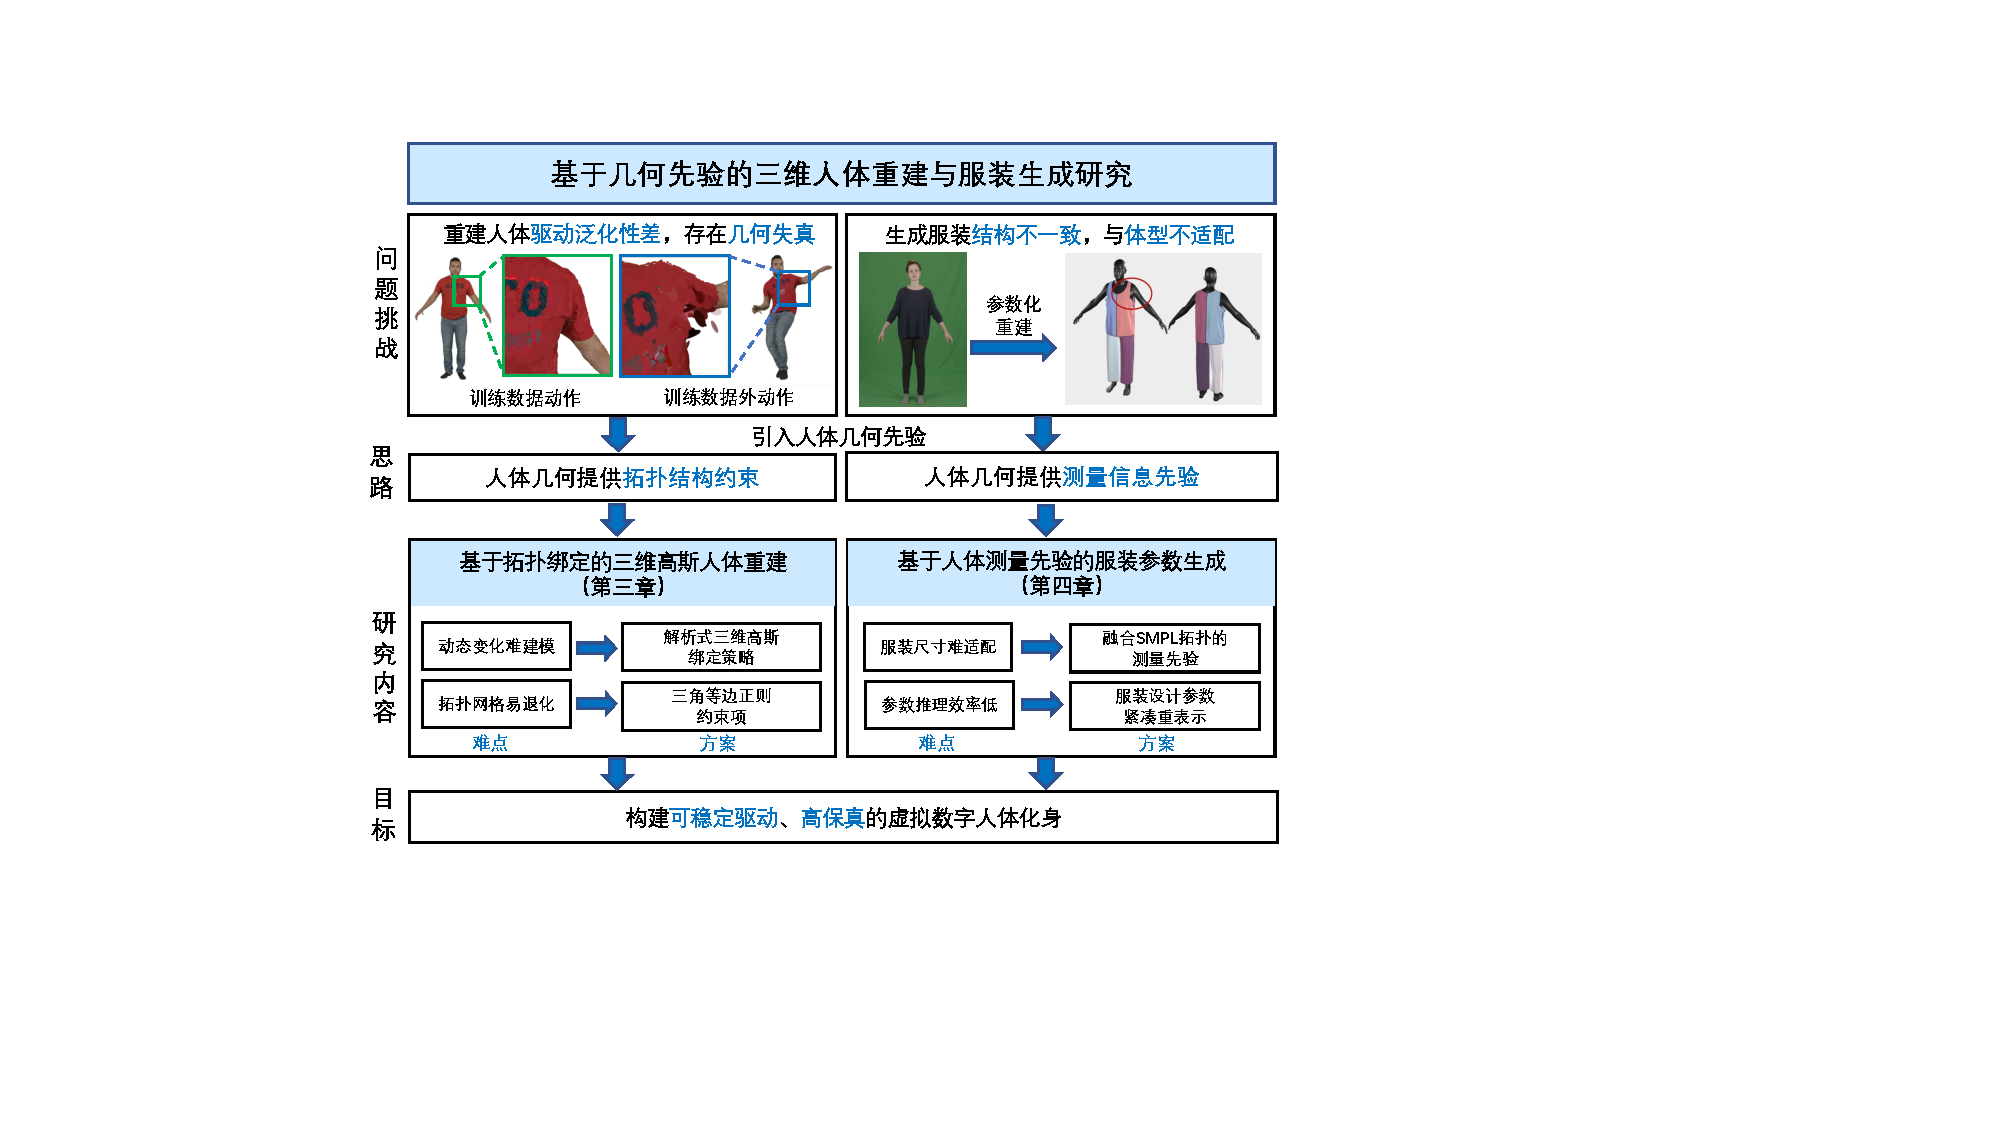
\includegraphics[width=0.85\linewidth]{main/chapter1/figures/example-figure.pdf}
    \caption{示例插图：实验结果可视化（请替换为你的图片）}
    \label{fig:ch4-example}
\end{figure}

\section{讨论与分析}

请在此分析实验结果背后的原因，讨论方法的优势、局限性与适用场景。如有必要，可补充消融实验、参数敏感性分析或失败案例分析。

\section{本章小结}

本章给出了实验设置、定量与定性结果，并对实验现象进行了讨论与分析。
